\documentclass[preprint,10pt]{sigplanconf}
\usepackage[boxed, ruled, noline, noend]{algorithm2e}
%\usepackage[letterpaper,left=0.75in,right=0.75in,top=1in,bottom=1in]{geometry}
%\usepackage[small,compact]{titlesec}
\usepackage{etoolbox}

\makeatletter
\patchcmd{\ttlh@hang}{\parindent\z@}{\parindent\z@\leavevmode}{}{}
\patchcmd{\ttlh@hang}{\noindent}{}{}{}
\makeatother
\usepackage[font={small,bf}]{caption}    % added 9/10/13
%\usepackage[nolineno,noindent,norules]{lgrind}
\usepackage{tightenum}
\usepackage{float}
\usepackage{xspace}
\usepackage{times,pifont}
\usepackage{mathptmx}
\usepackage{subfig,graphics,graphicx,color}
\usepackage{multirow}
\usepackage{dblfloatfix} %% correctly orders single- and double-col figures
%\usepackage{hyphenat}
\usepackage{mathrsfs}
\usepackage{subfig}
\usepackage{amssymb,amsmath,centernot}
\usepackage{lastpage}
\usepackage{flushend}
\usepackage{hhline}
\usepackage{authblk}
\usepackage{pifont}
\usepackage{listings}
\usepackage[hyphens]{url}
\usepackage{booktabs}
%\newcommand{\doi}{XXXXXX}


\frenchspacing


%%%%%%%%%%%%%%%%%%%%%%%%%%%%
%     macro

\newcommand{\xxx}[0]{\textsc{Owl}\xspace}
\newcommand{\paxos}[0]{\textsc{Paxos}\xspace}
\newcommand{\mytitle}[0]{\textbf {Understanding and Detecting Concurrency 
Attacks}}
\newcommand{\mykeywords}[0]{State Machine Replication, Fault Tolerance, Stable 
and Deterministic Multithreading, Software Reliability}

%%%%%%%%%%%%%%%%%%%%%%%%%%%%%%%%%%%%%%%%%%%%%%%%%%%%%%%%%%%%%%%%%
% hyperref stuff

%\usepackage[square,comma,numbers,sort]{natbib}
%\usepackage{hypernat}
%\usepackage{hyperref}

%% fill in pdf info here
%\hypersetup{%
%colorlinks=false,
%pdfborder={0 0 0},
%pdftitle={\mytitle},
%pdfkeywords={\mykeywords},
%bookmarksnumbered,
%pdfstartview={FitH},
%urlcolor=cyan,
%pdfpagelabels=true,
%pdfdisplaydoctitle=true,
%}%

%\usepackage{breakurl}
%\usepackage[all]{hypcap}
%\renewcommand{\url}{\burl}

%%%%%%%%%%%%%%%%%%%%%%%%%%%%%%%%%%%%%%%%%%%%%%%%%%%%%%%%%%%%
% Some NICE fonts

\newfont{\BIG}{cminch}                             %--- One-inch font
\newfont{\sfbHuge}{cmssbx10 scaled\magstep5}       %-- 25pt sans serif bold
\newfont{\sfbLarger}{cmssbx10 scaled\magstep3}   %-- 12+pt sans serif boldd
\newfont{\sfblarger}{cmssbx10 scaled\magstep2}   %-- 12+pt sans serif bold
\newfont{\sfblarge}{cmssbx10 scaled\magstep1}      %-- 12pt sans serif bold
\newfont{\sfbeleven}{cmssbx10 scaled\magstephalf}  %-- 11pt sans serif bold
\newfont{\sfb}{cmssbx10}                           %-- 10pt sans serif bold
\newfont{\sfeight}{cmss8}                          %-- 8pt sans serif

%%%%%%%%%%%%%%%%%%%%%%%%
%    space tweaking

%\textwidth = 6.5 in
%\textheight = 9.0 in
%\setlength{\topmargin}{-.5in}

%\headheight = 0.0 in
%\headsep = 0.0 in
%\parskip = 0.2in
%\parindent = 0.0in


%\renewcommand{\topfraction}{0.95}
%\addtolength{\textfloatsep}{-0.1in}
%\addtolength{\floatsep}{0.025in}
%\renewcommand\floatpagefraction{.9}
%\renewcommand\bottomfraction{.9}
%\renewcommand\textfraction{.1}

%\setlength{\parindent}{9pt}

% Rescue
\makeatletter
\def\v#1{{\mbox{\fontfamily{cmtt}\fontsize{\f@size}{\f@size}\selectfont #1}}}

\newcommand{\cmark}{\ding{51}}%
\newcommand{\xmark}{\ding{55}}%


\newcommand{\dmt}[0]{DMT\xspace}
\newcommand{\smt}[0]{StableMT\xspace}
\newcommand{\smr}[0]{SMR\xspace}

\newcommand{\tsan}[0]{\textsc{TSan}\xspace}
\newcommand{\valgrind}[0]{\textsc{Valgrind}\xspace}
\newcommand{\ski}[0]{\textsc{Ski}\xspace}
\newcommand{\lldb}[0]{\textsc{LLDB}\xspace}
\newcommand{\racepro}[0]{\textsc{RacePro}\xspace}
\newcommand{\criu}[0]{\textsc{CRIU}\xspace}
\newcommand{\lxc}[0]{\textsc{LXC}\xspace}
\newcommand{\tern}[0]{\textsc{Tern}\xspace}
\newcommand{\peregrine}[0]{\textsc{Peregrine}\xspace}
\newcommand{\parrot}[0]{\textsc{Parrot}\xspace}
\newcommand{\repframe}[0]{\textsc{RepFrame}\xspace}
\newcommand{\grace}[0]{Grace\xspace}
\newcommand{\coredet}[0]{\textsc{CoreDet}\xspace}
\newcommand{\kendo}[0]{Kendo\xspace}
\newcommand{\dthreads}[0]{\textsc{DThreads}\xspace}
\newcommand{\determinator}[0]{Determinator\xspace}
\newcommand{\dos}[0]{dOS\xspace}
\newcommand{\ddos}[0]{DDOS\xspace}
\newcommand{\timealgo}[0]{time bubbling\xspace}
\newcommand{\ldpreload}[0]{LD\_PRELOAD\xspace}
\newcommand{\ntimeout}[0]{$W_{timeout}$\xspace}
\newcommand{\nclock}[0]{$N_{clock}$\xspace}

\newcommand{\windows}{\v{Windows}\xspace}
\newcommand{\chrome}{\v{Chrome}\xspace}
\newcommand{\moonlight}{\v{Moonlight}\xspace}
\newcommand{\linux}{\v{Linux}\xspace}
\newcommand{\macos}{\v{Mac OS}\xspace}
\newcommand{\ios}{\v{iOS}\xspace}
\newcommand{\darwin}{\v{Darwin}\xspace}
\newcommand{\iexplorer}{\v{IE}\xspace}
\newcommand{\libsafe}{\v{Libsafe}\xspace}
\newcommand{\libvirt}{\v{Libvirt}\xspace}
\newcommand{\freebsd}{\v{FreeBSD}\xspace}
\newcommand{\kde}{\v{KDE}\xspace}
\newcommand{\ssdb}{\v{SSDB}\xspace}
\newcommand{\apache}{\v{Apache}\xspace}
\newcommand{\mysql}{\v{MySQL}\xspace}
\newcommand{\mongoose}[0]{\v{Mongoose}\xspace}
\newcommand{\ab}{\v{ApacheBench}\xspace}
\newcommand{\clamav}{\v{ClamAV}\xspace}
\newcommand{\upnp}{uPnP\xspace}
\newcommand{\mediatomb}{\v{MediaTomb}\xspace}
\newcommand{\memcached}{\v{Memcached}\xspace}
\newcommand{\mencoder}{\v{mencoder}\xspace}
\newcommand{\mongodb}{\v{MongoDB}\xspace}
\newcommand{\sysbench}{\v{SysBench}\xspace}
\newcommand{\zookeeper}{\v{ZooKeeper}\xspace}


\newcommand{\aget}[0]{\v{aget}\xspace}
\newcommand{\pthread}[0]{\mbox{Pthreads}\xspace}
\newcommand{\openldap}[0]{{OpenLDAP}\xspace}
\newcommand{\redis}[0]{{Redis}\xspace}
\newcommand{\bdb}[0]{{Berkeley DB}\xspace}
\newcommand{\vtune}[0]{\v{VTune}\xspace}
\newcommand{\http}[0]{\mbox{HTTP}\xspace}

% In short.
\newcommand{\eg}{{e.g.}}
\newcommand{\ie}{{i.e.}}
\newcommand{\etc}{{etc}}
\newcommand{\para}[1]{\vspace{.00in}\noindent{\bf #1}}
\newcommand{\wrt}{{w.r.t. }}
\newcommand{\cf}{{cf. }}

% Synch and network operations.
\newcommand{\checktimebubble}[0]{\v{check\_add\_timebubble()}\xspace}
\newcommand{\mutexlock}[0]{\v{pthread\_mutex\_lock()}\xspace}
\newcommand{\connect}[0]{\v{connect()}\xspace}
\newcommand{\send}[0]{\v{send()}\xspace}
\newcommand{\sendto}[0]{\v{sendto()}\xspace}
\newcommand{\sendmsg}[0]{\v{sendmsg()}\xspace}
\newcommand{\mywrite}[0]{\v{write()}\xspace}
\newcommand{\pwrite}[0]{\v{pwrite()}\xspace}
\newcommand{\close}[0]{\v{close()}\xspace}
\newcommand{\recv}[0]{\v{recv()}\xspace}
\newcommand{\select}[0]{\v{select()}\xspace}
\newcommand{\poll}[0]{\v{poll()}\xspace}
\newcommand{\epollwait}[0]{\v{epoll\_wait()}\xspace}
\newcommand{\accept}[0]{\v{accept()}\xspace}
\newcommand{\uselib}[0]{\v{uselib()}\xspace}
\newcommand{\mmap}[0]{\v{mmap()}\xspace}

% Parrot primitives.
\newcommand{\getturn}[0]{\v{get\_turn()}\xspace}
\newcommand{\putturn}[0]{\v{put\_turn()}\xspace}
\newcommand{\wait}[0]{\v{wait()}\xspace}
\newcommand{\signal}[0]{\v{signal()}\xspace}

% Evaluation stats.
\newcommand{\github}[0]{\url{github.com/asplos17-paper82/owl}}
% \newcommand{\ntype}[0]{four\xspace}
\newcommand{\nprog}[0]{10\xspace}
\newcommand{\nextraattacks}[0]{XX\xspace}
\newcommand{\nattacks}[0]{26\xspace}
\newcommand{\nconfirmed}[0]{15\xspace}
\newcommand{\nreproduced}[0]{10\xspace} % Concurrency attacks that we reproduced
\newcommand{\nreproducedProgs}[0]{6\xspace}
\newcommand{\nreproducedNoRetry}[0]{8\xspace}
\newcommand{\nreproducedInter}[0]{7\xspace}
\newcommand{\napacheDetected}[0]{783\xspace} % race report number of apache
\newcommand{\nmysqlDetectedSameReq}[0]{202\xspace} % race report number of 
% mysql on same req
\newcommand{\nmysqlDetected}[0]{1123\xspace} % race report number of mysql
% \newcommand{\apacheoverflowvalue}[0]{\verb!12345678!}
\newcommand{\nbackendDetected}[0]{10\xspace} % Concurrency attacks that backend is able to detect
\newcommand{\nevalProg}[0]{9\xspace}
\newcommand{\nbuggyProg}[0]{2\xspace}
\newcommand{\nvulnerableProg}[0]{4\xspace}
\newcommand{\nunknownVulUnknownBug}[0]{1\xspace}
\newcommand{\nunknownVulknownBug}[0]{3\xspace}
\newcommand{\numNewAttacks}[0]{3\xspace}
\newcommand{\nraces}[0]{16049\xspace} % Number of raw race reported by tsan
\newcommand{\nknownBugProg}[0]{5\xspace} % Number of programs evaluated with known bugs
\newcommand{\nnew}[0]{4\xspace}
\newcommand{\nknownVul}[0]{7\xspace}
\newcommand{\nunknownVul}[0]{3\xspace}
\newcommand{\reducerate}[0]{94.3\%\xspace}
\newcommand{\nadhocsync}[0]{22\xspace}
\newcommand{\ncustomizedsync}[0]{88\xspace}


\def\LGfsize{\footnotesize}
%\pagestyle{empty}


\begin{document}
\title{\mytitle}
%\setlength{\columnsep}{0.25in}
% \authorinfo{XXX}{YYY}

\authorinfo{Paper \#82}{The University of Hong Kong}{@cs.hku.hk}
% \author[*]{Rui Gu}
% \author[*]{Cheng Liu}
% \author[x]{Tianyu Chen}
% \author[*]{Junfeng Yang}
% \setlength{\affilsep}{0.5em}
% \renewcommand\AB@affilsepx{\hspace{28.0 mm}\protect\Affilfont}
% \affil[+]{\textrm\fontsize{10}{10}\selectfont The University of Hong Kong}
% \affil[*]{\textrm Columbia University}
% \affil[x]{\textrm Tsinghua University\vspace{-7.0 mm}}


% Hack for: Package caption Error: No float type 'copyrightbox' defined.
%\newcounter{copyrightbox}

\date{}

%\author[+]{\hspace{0 mm}\fontsize{10}{10}\selectfont Paper 247, SOSP 2015}
\maketitle
%\thispagestyle{empty}

\begin{sloppypar}
\begin{abstract}
Just like sequential bugs lead to attacks, concurrency bugs also lead to concurrency attacks. 
\end{abstract}
\end{sloppypar}

% \begin{sloppypar}
%% %\category{D.2.5}{Software Engineering}{Testing and Debugging}
%% \category{D.4.5}{Operating Systems}{Threads, Reliability}
%% \category{D.2.4}{Software Engineering}{Software/Program Verification}
%% \terms{Algorithms, Design, Reliability, Performance}
%% \keywords{\mykeywords}

%% \vskip 2mm
%% \noindent {\small \bf Categories and Subject Descriptors:} \vskip -.2mm
%% \noindent
%% {\footnotesize D.4.5~[{\bf Operating Systems}]: {Threads, Reliability}\\
%% D.2.4~[{\bf Software Engineering}]: {Software/Program Verification};}
%% \vskip 1mm
%% \noindent {\small \bf General Terms:} \vskip -.2mm
%% \noindent
%% {\footnotesize Algorithms, Design, Reliability, Performance}
%% \vskip 1mm
%% \noindent {\small \bf Keywords:} \vskip -.2mm
%% \noindent
%% {\footnotesize \mykeywords}

% \vskip 2mm
% \noindent {\small \bf Categories and Subject Descriptors:}
% {\small D.4.5~[{\bf Operating Systems}]: {Threads, Reliability};
%   D.2.4~[{\bf Software Engineering}]: {Software/Program Verification};}
% \vskip .1mm
% \noindent {\small \bf General Terms:} {\small Algorithms, Design,
%   Reliability, Performance}
% \vskip .1mm
% \noindent {\small \bf Keywords:} {\small \mykeywords}
% 
% \end{sloppypar}

%%%%%%%%%%%%%%%%%%%%%%%%%%%%%%%%%%%
% Add page number.
\setcounter{page}{1}
\pagenumbering{arabic}

\thispagestyle{plain}
\pagestyle{plain}
\setlength{\footskip}{20pt}
%%%%%%%%%%%%%%%%%%%%%%%%%%%%%%%%%%%

%\begin{sloppypar}

%\vskip 2mm
%\noindent {\small \bf Categories and Subject Descriptors:}
%{\small D.4.5~[{\bf Operating Systems}]: {Threads, Reliability};
  %C.2.4~[{\bf Computer-communication Networks}]: {Distributed Systems};}
%\vskip .1mm
%\noindent {\small \bf General Terms:} {\small Algorithms, Design,
  %Reliability, Performance}
%\vskip .1mm
%\noindent {\small \bf Keywords:} {\small \mykeywords}

%\end{sloppypar}

\begin{sloppypar}

\section{Introduction} \label{sec:intro}


%1. Interleaving - crash - explicit behaviour - 
Multi-threaded program is hard to be correct. 
Concurrency bugs are common in modern multi-threaded programs  
including atomic violation, ..., and especially data race\cite{lu:concurrency-bugs,conmem:asplos10,conseq:asplos11, lu:muvi:sosp}.
Extant work well explores interleaving that causes concurrency bugs, 
and efficiently detects explicit concurrency bugs that direct to  
severe consequences such as execution order violation, wrong output and program crash
\cite{wu2015:collaborative,tsan,valgrind:pldi,lu:muvi:sosp,conseq:asplos11,conmem:asplos10}.
%and by employing memory sanitizers and thread sanitizers, severe concurrency bugs
%may be explicit(?..).

%2. Recent study - con attacks - structural , consequence, [in-explicit severer]
Recent studies\cite{acidrain:sigmod17,con:hotpar12} show rise of concerns about \emph{concurrency attacks}.
Just like sequential bugs lead to attacks, concurrency bugs also lead to concurrency attacks. 
By triggering concurrency bugs and employing subtle inputs, 
hackers may leverage the corrupted memory to conduct  
attacks including privilege escalations\cite{uselib-bug-12791,mysql-bug-14747}, hijacking code execution\cite{berend-jan-wever-msiexploit}, bypassing security checks\cite{xwindows,theotheriphone,theotheriphone-2011}, 
and breaking database integrity\cite{acidrain:sigmod17}.
These vulnerabilities often hide in large amount of concurrency bug reports. 
For example, bug information leveraged by a xxx attack is hidden in 1000 race reports 
produced by TSAN\cite{tsan}, a famous and widely used data race detector. 
%Also, to construct concurrency attacks, despite the inputs of leveraged concurrency bugs, 
%attacker may need other crafted inputs to exploit the vulnerabilities. 
***Also, despite threads conducting concurrency bugs, 
behaviors of another thread may also be affected when data race bugs infecting shared memory (\eg heap overflow)\cite{apache-bug-25520,cve:2017-7533}. ***


%3. Unfortunately, most extant work -- detect bug, corruption 
%   Our study - old bug - attack
%   However in danger
%   Sigmod 
Unfortunately, although great progress has been made to detect and replay severe bugs(\eg ConMem\cite{conmem:asplos10}), 
extant work still lacks exploration of concurrency attacks from enormous concurrency bugs. Our study over several known concurrency 
bugs\cite{apache-bug-25520, apache-bug-46215} shows that even concurrency bugs have been successfully detected and reported, 
professionals may still lack knowledge about how severe consequences these bugs may cause. 
For instance, \emph{apache-25520}\cite{apache-bug-25520} has been 
reported over years and well studied by researchers\cite{lu:concurrency-bugs}.  
We are the first to exploit a new heap overflow attack leveraging on this bug and break the HTML integrity.  

%4. Two major challenges : 
%a. concurrent bug detectors (justify) 
%b. other input for attack
We studied \nattacks attacks and find two major challenges for exploring concurrency attacks from concurrency bugs. 
First, concurrency attacks may be implicit and hidden in common concurrency bugs. 
Existing concurrent bug detectors focus on bug happening itself. 
ConMem\cite{conmem:asplos10} first propose to 
consider concurrency bugs that may cause severe consequences (\eg program crash)
and ConSeq\cite{conseq:asplos11} uses severe consequence report to help diagnose concurrency bugs. 
However, our observation shows that explicit error (\eg program crash) is not necessary for concurrency 
attacks. Some concurrency bugs (\eg \emph{xxx-xxx}) may not cause program crash or interrupted, 
but attackers may still leverage them and conduct attacks with crafted input. 
%Here the propagation path?
%
???-Worse still, crash bugs may even lead to more severe vulnerabilities. 
In \emph{CVE-2017-7533} conducted by our team, although the data race primarily causes kernel crash, 
we crafted the input and successfully conduct a privilege escalation attack without crashing the kernel.
Current concurrency bug detecting tools are not designed to analyze this kind of latent vulnerabilities, 
and hence may direct wrong level of warnings towards the bugs.  


Second, extant work ignores indicating the \emph{victim thread} of concurrency attacks.
A concurrency bug may become much more vulnerable when attackers employee another thread to construct 
their attacks. 
In CVE-2017-7533, we do not only leverage two threads to trigger a data race and construct kernel heap overflow, 
but also require another \emph{victim thread} to lay the target structure on the same heap. 
By crafting inputs and corrupting the target structure, we finally achieve arbitrary code execution and get a root shell. 
Automatically indicating the victim thread would be of vital helpful for developers to better understand the latent vulnerabilities.
For example, in the Apache-25520 case, after knowing about information of victim thread, 
we successfully increased the severity of the bug and conducted an integrity violation.

%5. New model for general attacks [] -- *vulnerability window 

To address the two challenges, we introduced a new model(\S\ref{sec:model}) 
that explains most concurrency attacks we studied. 
The model breaks down concurrency attacks into three stages: bug happening, 
bug-to-attack propagation, and attack happening. In this model, 
the two key things for exploring concurrency attacks is 
the analysis of bug-to-attack propagation and definition of attack happening, 
while bug happening has been well studied and detected. Our studies show propagation 
includes data flow and  



%6. Leveraging this model, framework - address two challenges.
Leveraging this model, we designed a two-phase framework(\S\ref{sec:archi}), \xxx, for detecting concurrency attacks. 
%7. Two phase. 
The first phase is \emph{concurrency analyzer} to analyze bug-to-attack propagations. 
Our study found that most vulnerable races are already included in the race detectors’ reports, 
and concurrency attacks sites are often explicit in program code.
Therefore, we can perform static analysis
on only the data and control flow propagations between the
bug reports and the potential attack sites, then we can collect
relevant call stacks and branch statements as the potentially
vulnerable input hints.

The second phase is \emph{concurrency fuzzer?} to ... .

%9. Implementation / CVE . reduction
We implemented \xxx on Linux, supporting both user space and kernel space attack detection. 



We evaluated OWL on 6 diverse, widely used programs, including Apache, Chrome, Libsafe, Linux kernel, MySQL,
and SSDB. OWL’s benign schedule hints and runtime verifiers reduced 94.3\% of the race reports, 
and it did not miss the evaluated concurrency attacks. With the greatly reduced reports,
OWL’s vulnerable input hints helped us identify subtle
vulnerable inputs, leading to the detection of 7 known concurrency
attacks as well as 3 previous unknown, severe ones
in SSDB and Apache. The analysis performance of OWL was
reasonable for in-house testing.


%10. Contribution
%     new model/ system / General -extension- .. new CVE..
This paper makes two major contributions:

\begin{tightenum}
\item \textbf{A general model explains happening and exploiting of concurrency attacks.} 
This model explains most concurrency attacks in wild and 
providing two major direction for detecting concurrency attacks. 
	
\item \textbf{A general concurrency attack detection framework and its implementation, \xxx.} 
\xxx can easily employ existing concurrent bug detectors and vulnerability analyzer 
to improve the accuracy and ??? of detection.
	
\end{tightenum}

 

%11. The rest of section
The rest of this paper is structured as follows. 
\S\ref{sec:background} introduces the background of concurrency attacks.
\S\ref{sec:overview} gives an overview on the concurrency attack model and architecture of \xxx.
\S\ref{}...






\section{Background}\label{sec:background}

% Prior study. Summary. Three major findings.
A prior study~\cite{con:hotpar12} browsed the bug databases of 46 real-world 
concurrency bugs and made three major findings on concurrency attacks. First, 
concurrency attacks are severe threats: 35 of the bugs can corrupt critical 
memory and cause three types of violations, including 
privilege escalations~\cite{uselib-bug-12791, mysql-bug-24988}, malicious code 
injections~\cite{berend-jan-wever-msiexploit}, and
bypassing security 
authentications~\cite{xwindows,theotheriphone,theotheriphone-2011}.

Second, concurrency bugs and attacks can often be easily triggered via subtle 
program inputs. For instance, attackers can use inputs to control the physical 
timings of disk IO and program loops and trigger concurrency bugs with a small 
number of re-executions. Third, compared to traditional TOCTOU attacks, which 
stem from corrupted file accesses, handling concurrency attacks is much more 
difficult because they stem from corrupted, miscellaneous memory accesses.

% Ineffectiveness of existing defense techniques.
These three findings reveal that concurrency attacks can largely weaken or 
even bypass most existing security defense tools, because these 
tools are mainly designed for sequential attacks. For instance, consider taint 
tracking tools, concurrency attacks can corrupt the metadata fields in these 
tools and completely bypass taint tracking. Anomaly detection tools, which rely 
on inferring adversary program behaviors (\eg, excessive re-executions), 
become ineffective, because concurrency attacks can easily manifest via subtle 
inputs.

% Introduce the question: what tool? Should be more directed here because the 
% prior study has shown the severity of concurrency attacks.
This prior study raises an open research question: \emph{what will be an 
effective tool for detecting concurrency attacks?} Specifically, can existing 
concurrency bugs detection tools effectively detect these bugs and their 
attacks? The answer is probably ``NO" because literature has overlooked these 
attacks.


\section{Quantitative Concurrency Attack Study}\label{sec:study}

% Study methodology. Studied XX real-world programs, including both applications 
% and kernels. Search CVE and open source bug databases with keywords. Manually 
% inspect the vulnerabilities. Use detection tools to detect these bugs if they 
% work with existing popular detection tools' platform (in total there are XX), 
% and inspected the number of total race reports, and inspect whether the race 
% reports have vulnerability implications.


% Our study, exclude tocttou, exclude repeated ones, added XX extra attacks, 
% finally identify 27 attacks.

We studied concurrency attacks in \nprog widely used programs, including 3 
servers, 2 browsers, 1 library, and 4 kernel distributions. We 
added the shared memory concurrency bugs in the prior 
study~\cite{con:hotpar12}, and we searched ``concurrency bug vulnerability" in 
CVE and these programs' bug databases. We manually inspected bug reports 
and removed them if they were false reports or lack a clear description, and 
we conservatively kept the vulnerable ones caused by multithreading.

Unlike the prior study~\cite{con:hotpar12} which counted the number of 
security consequences in bug reports as the number of concurrency attacks, 
we counted only each bug's first security consequence. In total we collected 
\nattacks concurrency attacks with three more types of violations than the 
prior study~\cite{con:hotpar12}, including HTML integrity violations 
(\S\ref{sec:unknown-attacks}), buffer overflows (\S\ref{sec:example}), and DoS 
attacks (\S\ref{sec:unknown-attacks}). We built scripts to successfully exploit 
\nreproduced attacks in \nreproducedProgs programs if we had source code.

To quantitatively analyze why concurrency attacks are overlooked, we  
considered data race detectors because they have effectively 
found concurrency bugs. We selected two popular tools: \tsan~\cite{tsan:wbia09} 
for applications and \ski~\cite{ski:osdi14} for OS kernels. We ran the two 
tools on \nreproducedProgs programs that support these tools. We used the 
programs' common performance benchmarks as workloads. 
Table~\ref{tab:study} shows a study summary.
% Our study also considerfed bug 
% consequence analysis tools and anomaly detection tools. 

% Prog order: from app to kernel; in app, from server to others; alphabetical.
\begin{table}[h]
\footnotesize
\centering
\vspace{-.1in}
\begin{tabular}{lrrrr}
{\bf Name} & {\bf LoC}  & {\bf \# Concurrency attacks}  & 
{\bf \# Race reports} \\
\hline\\[-2.3ex]
% apps
%\moonlight                &    TBD   &    1 &    N/A \\
%\kde                      &    TBD   &    2 &    N/A \\
% kernels
%\macos                    &    TBD   &    2 &    N/A \\
\apache                     &    290K  &    4 &    715  \\
\mysql                      &    1.5M  &    2 &    1123 \\
\ssdb                       &    67K   &    1 &    12  \\
\chrome                     &    3.4M  &    3 &    1715 \\
\iexplorer                  &    N/A   &    1 &    N/A \\
\libsafe                    &    3.4K  &    1 &    3   \\
% \libvirt                    &    680K  &    1 &    0 \\
\linux                      &    2.8M  &    8 &    24641 \\
\darwin                     &    N/A   &    3 &    N/A \\
\freebsd                    &    680K  &    2 &    N/A \\
\windows                    &    N/A   &    1 &    N/A \\
\hline\\[-2.3ex]
Total                       &    8.0M  & \nattacks & 28209 \\
\end{tabular}
\vspace{-.1in}
\caption{{\em Concurrency attacks study results.} \rm {This table contains both 
known and previously unknown concurrency attacks we detected. We 
made \nreproducedProgs out of \nprog programs run with race 
detectors. We built exploit scripts for \nreproduced concurrency 
attacks in these \nreproducedProgs programs.}} 
\label{tab:study}
\vspace{-.15in}
\end{table}



\subsection{Challenging Findings}\label{sec:findings}



%\begin{figure}[h]
%\centering
%\includegraphics[width=0.8\columnwidth]{figures/apache}
%%\vspace{-.1in}
%\caption{{A concurrency attack in the \apache web server.}} \label{fig:apache}
%\vspace{-.15in}
%\end{figure}



% These attacks allow attackers to 
% corrupt critical memory, overflow heaps and stacks, inject malicious code, 
% escalate programs' privileges, and bypass authentication checks. 

\para{I: Concurrency attacks are much more severe than concurrency bugs.} Every 
studied program has concurrency attacks. Figure~\ref{fig:libsafe} shows a 
concurrency attack that bypassed stack overflow checks in the 
\libsafe~\cite{libsafe} library and injected malicious 
code. Figure~\ref{fig:uselib} shows a concurrency attack in the Linux \uselib 
system call. Attackers have leveraged this bug to trigger a NULL pointer 
dereference in the kernel and execute arbitrary code from user space.

One key difference between concurrency attacks and concurrency 
bugs is that fixing the buggy code is not sufficient to fix the 
vulnerabilities. For instance, once attackers have got OS root 
privileges~\cite{freebsd-exploit-2009-3527,uselib-bug-12791}, they may stay 
forever in the system. Therefore, it's still crucial to study whether existing 
known concurrency bugs may lead to concurrency attacks.

\begin{figure}[h]
\vspace{-.1in}
\centering
\includegraphics[width=0.8\columnwidth]{figures/libsafe}
\vspace{-.55in}
\caption{{A concurrency attack in the \libsafe security library. } 
\rm{Dotted arrows mean the bug-triggering thread interleaving. When Thread 2 
detects a stack overflow attack, it sets the \v{dying} variable to 1 and kills 
current process shortly. However, access to \v{dying} is not correctly 
protected 
by mutex, so Thread 1 reads this variable, bypasses the security check in
\v{stack\_check()} (called at line 164), and runs into a 
stack overflow in \v{strcpy()} (at line 165).}}
\label{fig:libsafe}
\end{figure}

\begin{figure}[h]
\centering
% \vspace{-.03in}
\includegraphics[width=0.9\columnwidth]{figures/kernel_uselib_msync}
\vspace{-.25in}
\caption{{A concurrency attack in the Linux \uselib and \v{msync()} system 
calls. }\rm{Dotted arrows mean the bug-triggering thread interleaving. A data 
race on the \v{f\_op} struct causes the Linux kernel to trigger a NULL 
pointer dereference and enables arbitrary code execution.}} 
\label{fig:uselib}
\vspace{-.1in}
\end{figure}

%\para{Concurrency attacks are more than just TOCTOU attacks.}
%Concurrency attacks are much broader than the TOCTOU attacks
%studied by previous work due to two main reasons. First, the TOCTOU attacks in 
%previous work target primarily the file access interface (\eg, \v{open()} 
%and \v{access()}). This interface allows users to check file permissions and 
%use file data but does not directly support transactions that make the check and 
%the use atomic. An attacker may thus exploit this limitation to gain illegal 
%file accesses. In contrast, the concurrency attacks we studied target general 
%memory access interface (\eg, \v{load} and \v{store} instructions), corrupt a 
%program's global memory (\eg, via data races), and lead to various types of 
%vulnerabilities.

% Heming: don't mention many buggy patterns because our front ends only have 
% data race detectors for now.
% Second, the TOCTTOU races in previous work exhibit one specific interleaving 
% pattern: atomicity violations where the check and the use is not atomic. In 
% contrast, our study reveals various interleaving patterns, including data 
% races, atomicity violations, order violations [25] where a set of accesses
% is supposed to occur in a fixed order, but no synchronizations
% % enforce the order.

%Second, as a natural fallout of the first reason, techniques proposed by 
%previous TOCTOU work are too specific to detect or prevent general concurrency 
%attacks. For instance, while launching a TOCTOU attack requires concurrent 
%executions, the vulnerable program may be purely sequential, so TOCTOU 
%detectors may not need to reason about concurrency at all. Similarly,
%TOCTOU detectors may mediate all file system calls without high runtime 
%overhead, but it would be prohibitive to mediate all load or store 
%instructions to detect data races.

\para{II: Concurrency bugs and their attacks are widely spread in program 
code.} Among \nreproduced attacks we had source code and constructed exploit 
scripts, \nreproducedInter have their bugs and vulnerability sites among 
different functions. Moreover, bugs often affect vulnerability sites not only 
through data flows but also control flows (\eg, the \libsafe attack in 
Figure~\ref{fig:libsafe}).

This finding suggests that a concurrency attack detection tool should 
incorporate both inter-procedural and control-flow analyses. Unfortunately, to 
scale to large programs, existing bug consequence analysis tools 
(\eg,~\cite{conseq:asplos11,yamaguchi:sp14,livshits05finding}) lack 
either inter-procedural or control-flow analysis.

\para{III: Concurrency bugs and their attacks are often triggered by separate, 
subtle program inputs.} Consider the inputs to trigger 
concurrency bugs, unlike previous 
understanding~\cite{pres:sosp09,cui:tern:osdi10} that 
triggering concurrency bugs require intensive repeated executions, 
\nreproducedNoRetry out of the
\nreproduced reproduced concurrency attacks in our study can be easily 
triggered with less than 20 repetitive executions on our evaluation machines 
with carefully chosen program inputs. For instance, in a \mysql 
privilege escalation~\cite{mysql-bug-24988}, we used the ``\v{flush 
privileges;}" query to trigger a data race and corrupted another \mysql user's 
privilege table with only 18 repeated executions.

In addition to input values, carefully crafted input timings can also expand 
the \emph{vulnerable window}~\cite{con:hotpar12} which increases the chance of 
running into the bug-triggering schedules. For 
instance, consider Figure~\ref{fig:uselib}, since the \v{if} statement and the  
\v{file->f\_op->fsync()} statement in \v{msync\_interval()} have an IO 
operation (not shown) in between, attackers could craft inputs with subtle timings 
for this IO operation and thus enlarged the time window of these two statements. 
Then, attackers could easily trigger the buggy schedule in Figure~\ref{fig:uselib}.

In addition to the inputs for triggering concurrency bugs, triggering the 
attacks of these bugs often require other subtle program inputs. A main 
reason is the bugs and their attacks are widely spread in program 
code and thus they may easily be affected by different inputs. In a Linux 
\uselib data race~\cite{uselib-bug-12791}, 
we needed to carefully construct kernel swap IO operations to trigger the race, 
and we needed to call extra system calls to get a root shell out of this race. 
By constructing subtle inputs for both the bug and its attack, we needed only 
tens of repeated executions to get this root shell on our evaluation machines.

This \uselib attack reveals two issues. First, a small number of repeated 
executions indicates that attackers can easily bypass anomaly detection 
tools~\cite{schonberg:pldi89,taskrecycling:ppopp90,diduce:icse02} 
with subtle inputs. Second, existing data race detectors are ineffective at 
revealing this attack because they will stop after they run a bug-triggering input 
and flag this race report. Such a one-shot detection will overlook a 
concurrency attack as it often requires extra inputs to trigger the attack. 
Therefore, extra analysis is required to identify the bug-to-attack propagation.

% TBD: heming, emphasis not only functions, but also indirect control flow 
% propagation. E.g., libsafe.
% TODO: Concurrency attacks are not necessarily only located in certain part of 
% the program code.

\para{IV: Most concurrency bugs that triggered concurrency attacks can be 
detected by race detection tools.} There are several types of concurrency bugs,
including data race, atomicity violation, 
and order violation~\cite{lu:concurrency-bugs}. Although some types of 
concurrency bugs are difficult to detect (\eg, order violation), we found that 
all concurrency bugs we studied were data races and these bugs can readily be 
detected by \tsan or \ski. This finding suggests that a race detector 
is a necessary component for detecting concurrency attacks.
% The only exception is the atomicity 
% violation bug in \libvirt (see Table~\ref{tab:study}). 

% This finding suggests 
% that data race detection tools should be a necessary component in a concurrency 
% attack detection system.

% Since the root cause of concurrency 
% attacks is concurrency bugs, it is vital to identify the associated concurrency 
% bugs in order to identify concurrency attacks. 
% However, not all types of 
% concurrency bugs can be detected by well used exisiting tools,

\para{V: Concurrency attacks are overlooked mainly due to the excessive 
reports from race detectors.} We identified two major reasons for this finding. 
First, existing race detectors generate too many bug reports which deeply bury 
the vulnerable ones. For instance, we ran \mysql with \tsan and repeatedly 
generated the same bug-triggering SQL query~\cite{mysql-bug-24988}. We got 
\nmysqlDetectedSameReq race reports, but after our manual inspection, only two 
reports will lead to attacks. Table~\ref{tab:study} shows 
more programs with even more reports. These excessive reports make 
finding concurrency attacks from the reports just like ``finding needles in a 
haystack."

Second, even if a developer luckily opens a true bug report that can actually 
lead to an attack, she still has no clue whether what attacks the bug may lead 
to, because the report only shows the bug itself (\eg, the corrupted variable), 
but not its security consequences. Therefore, it's crucial to have an analysis 
tool that can accurately identify the bug-to-attack propagation for bug reports.

% Heming: hack, make the arch figure locate at the same page as section 4.2.
\begin{figure*}[!tbh]
\centering
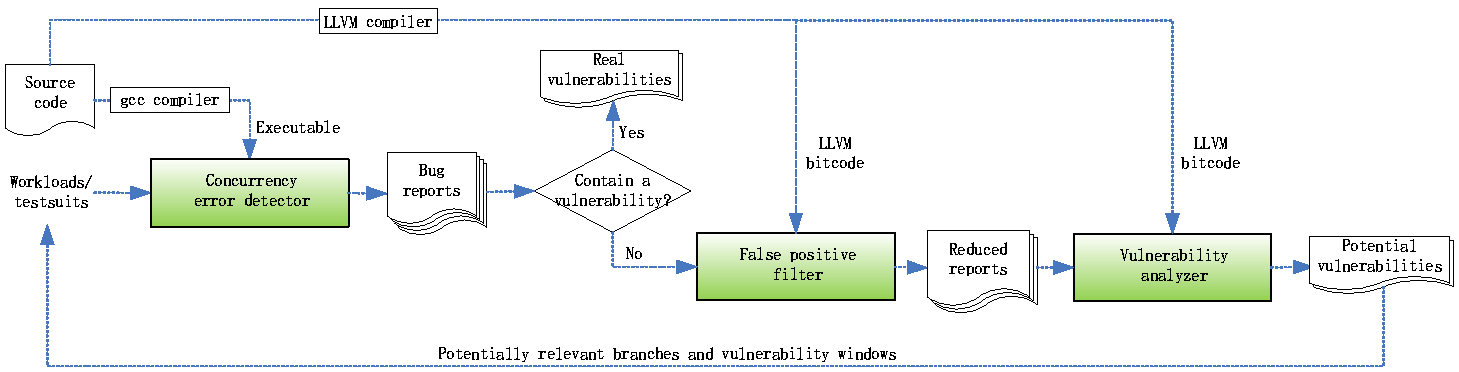
\includegraphics[width=0.7\textwidth]{figures/arch}
\vspace{-.20in}
\caption{{\em The \xxx Architecture.} \rm {\xxx components are the blue 
(shaded) ones.}} \label{fig:arch}
\vspace{-.2in}
\end{figure*}

\subsection{Optimistic Findings}\label{sec:patterns}

To assist the construction of a practical concurrency attack detection tool, 
we identified two common patterns for concurrency attacks. First, although the 
consequences of concurrency attacks are miscellaneous, these consequences are 
triggered by five explicit types of vulnerable sites, including memory 
operations (\eg, \v{strcpy()}), NULL pointer deferences, privilege operations 
(\eg, \v{setuid()}), file operations (\eg, \v{access()}), and process-forking 
operations (\eg, \v{eval()} in shell scripts). Our study found that these 
vulnerable sites have independent consequences to each other, thus more types 
can be easily added.


Second, concurrency bugs and their attacks often share similar call stack 
prefixes. From the \nreproduced concurrency attacks with source code, 
\nreproducedInter of them have the vulnerability site in the callees (\ie, the 
call stack of the bug is a prefix of the call stack of the vulnerability site). 
For the rest them, the vulnerability site is just one or two levels up of the 
bug's call stack. These two patterns reveal an opportunity to build a precise, 
scalable static analysis tool for tracking the bug-to-attack propagation.

% the corrupted memory of concurrency 
% attacks rarely propagate through return values of function calls. This is 
% probably due to the corrupted memory is global varible or heap, but not stack 
% variables. 

% First, because 
% concurrency attacks tend to leverage the corrupted memory that resides during a 
% program's execution, the propagation from the corrupted memory to a 
% vulnerability action widely 
% spreads across branch instructions and function calls. For instance, 5 
% concurrency attacks we studied incurred at least XX branch instructions or 
% function calls. This long propagation distance indicates that existing 
% consequence-oriented analysis tools (\eg,~\cite{conseq:asplos11}) for 
% concurrency bugs may work poorly on concurrency attacks.






\section{\xxx Overview}\label{sec:overview}

\section{Reducing Benign Schedules} \label{sec:schedule-reduction}

This section presents \xxx's benign schedule reduction component, 
including automatically annotating adhoc synchronizations 
(\S\ref{sec:adhoc-sync}) and pruning benign schedules 
(\S\ref{sec:verify-race}). This component in total greatly reduced 
\reducerate of the total reports (see \S\ref{sec:reduce}).

\subsection{Annotating Adhoc Synchronization} 
\label{sec:adhoc-sync}
% Busy loop filter.
Developers use semaphore-like adhoc synchronizations, where one thread is
busy waiting on a shared variable until another thread sets this variable to be
``true". This type of adhoc synchronizations couldn't be recognized by \tsan or 
\ski and caused many false positives.

\xxx uses static analysis to detect these synchronizations in two steps. First, 
by taking the race reports from detectors, it sees if the ``read" instruction 
is in a loop. Then, it conducts a intra-procedural forward data and control 
dependency analysis to find the propagation of the corrupted variable. If \xxx 
encounters a branch instruction in the propagation chain, it checks if this 
branch instruction can break out of the loop. Last, it checks if the ``write'' 
instruction of the instruction assigns a constant to the variable. If so, \xxx 
tags this report as an ``adhoc sync".

Compared to the prior static adhoc sync identification 
method SyncFinder~\cite{syncfinder:osdi10}, which finds the 
matching ``read'' and ``write'' instruction by statically searching program 
code, our approach leverages the actual runtime information from the race 
reports, so ours are much simpler and more precise.
% Evaluation confirmed that this filter can filter out 
% busy looping synchronization with a precision of 100\% by our manual inspection.

\subsection{Verifying Real Data Races}\label{sec:verify-race}

% Compensate the lack of pointer aliasing.
\xxx's dynamic race verifier checks whether the reduced race reports 
are indeed real races. It also generates security hints for the 
following analysis. The verifier is lightweight because it is built on top of 
the \lldb debugger. We find that a good way to trigger a data race is to catch 
it ``in the racing moment". The verifier sets thread specific breakpoints 
indicated by \tsan race reports. ``Thread specific" means when the breakpoint 
is triggered, we only halt that specific thread instead of the whole program. 
The rest of the threads are still able to run. In this way, we can actually 
catch the race when both of the racing instructions are reached by different 
threads and are accessing the same address.

% Currently, we are not aiming for completeness(ie. miss no bugs),
% rather our dynamic filter aims to provide sound results filtered from race 
% detector's reports by eliminating false positives.


%A script will extract filenames, line numbers from the reports and set thread
%specific breakpoints at the corresponding locations. 
%Once a breakpoint is hit within \lldb, our script will extract the address of
%the shared memory that the instruction is accessing. We’ll then create a tuple
%that contains \verb!(AccessedAddress, !\verb!InstructionType,! \verb!ThreadID)!.
%\verb!InstructionType! indicates where it’s the Read Instruction or the Write
%Instruction in the racing pair. It will store this tuple in a global array and
%suspend the thread.  Besides storing the info and suspend the thread, our tool
%will also compare this info to previous stored info of the other instruction in
%the racing pair from the other suspended threads in the global array.
%If there is a match, a match means the \verb!AccessAddress! are the same while 
%\verb!ThreadID!
%and \verb!InstructionType! are different, we know that both instructions can be 
%reached
%simultaneously by different threads and they’re accessing the same address.
For each run, \xxx's dynamic filter verifies one race. Once a data race is 
verified, the verifier goes one step further. It prints the following dynamic
information as security hints including, the racing instructions from source
code, the value they're about to read and write and the type of the variable
that these instructions are about to read or write. These hints show whether a 
NULL pointer difference can be triggered or an uninitialized data can be read 
because of the race.

It is possible that due to the suspension of threads, the program goes into a 
livelock state before verifying any data races. We resolve this livelock state
by temporarily releasing one of the currently triggered breakpoints. 

%In other to resolve livelock, we define two livelock states.\\
%{\bf State 1:}
%There isn’t any incoming breakpoints hit within certain time threshold.\\
%{\bf State 2:}
%All the executing threads are paused by our system.

%In the first case, if there is any suspended thread, we’ll pick one randomly
%and release that thread. Note that by saying release the thread, we don’t mean
%remove any breakpoints. So this released thread can still hit breakpoints in the
%future execution. The stored info in the global array will also be removed.
%If there isn’t any suspended threads, we will just terminate the whole program
%and move on to next data race that needs to be verified.
%In the second case, we will also randomly pick up one thread and release it.
%The records stored in the global array will also be removed at the same time.

%Overall, this livelock resolving mechanism prevents our verifier from becoming
%livelocked and maximize the chances in verifying data races for each run.
%When the system is halted, we only release one thread. In some circumstances,
%this action sequentialize the execution of the targeted program. We make this
%design choice because we choose to be conservative in order to maximize the 
%chance
%of verifying the racing pairs in the sacrifice of performance.

Previous works~\cite{racefuzzer, conbreak, conpredicates} adopt the same core
idea of “thread specific breakpoints” and
data race verification. \xxx's dynamic race verifier provides a lightweight,
general, easy to use way (integrated with existing debugger)
in verifying “potentially” harmful data races and their consequences.
Compared with RaceFuzzer~\cite{racefuzzer}, \xxx's verifier achieves the goal 
without requiring heavyweight Java instrumentation. Compared with
ConcurrentBreakpoint~\cite{conbreak} and ConcurrentPredicate~\cite{conpredicates},
we require no code annotations and importing libraries.

Overall, \xxx's dynamic filter makes developers be less dependent on 
the particular front end race detector, because no matter how many false 
positive the front end race detector generates, this verifier will make sure 
the end result is accurate.
% Our tool is sound.

% To achieve soundness, \xxx's verifier trades off completeness.
There are two cases that could cause \xxx's race verifier to miss real races. First, if the 
race detector doesn't detect the race upfront, the verifier won't report the 
race either. Second, depending on runtime effects (\eg, schedules), some races 
can't be reliably reproduced with 100\% success rate~\cite{conpredicates}.

\section{Computing Vulnerable Input Hints} \label{sec:input-reduction}

This section presents the algorithm of \xxx's static vulnerability 
analysis (\S\ref{sec:algo}) and dynamic verifier 
(\S\ref{sec:vulnerability_verifier}). Since the input of the static 
analysis is the reports from concurrency bug detectors, this section then 
describes how \xxx integrates this analysis with two existing race 
detectors (\S\ref{sec:integration}).

\subsection{Analysis Algorithm} \label{sec:algo}

\begin{algorithm}[t]

\DontPrintSemicolon

%\SetCommentSty{textrm}

\small

\SetCommentSty{textrm}

\SetKwInOut{Input}{Input}\SetKwInOut{Output}{Global}
\Input{program $prog$, start instruction $si$, $si$ call stack $cs$}
\Output{corrupted instruction set $crptIns$, vulnerability set $vuls$}

\SetKwBlock{Titlea}{DetectAttack($prog$, $si$, $cs$)}{end}
\Titlea {
  $crptIns$.add $si$ \;
  \While{$cs$ \rm is not empty} {
    $function$ $\leftarrow$ $cs$.pop \;
    $ctrlDep$ $\leftarrow$ false \;
    DoDetect($prog$, $si$, $function$, $ctrlDep$) \;
  }
}

\SetKwBlock{Titlea}{DoDetect($prog$, $si$, $function$, $ctrlDep$)}{end}
\Titlea {
  set $localCrptBrs$ $\leftarrow$ empty \;
  \ForEach {{\rm succeeded instruction $i$}} {
    bool $ctrlDepFlag$ $\leftarrow$ false\;
    \ForEach {{\rm branch instruction $cbr$ in $localCrptBrs$}} {
        \If {$i$ \rm is control dependent on $cbr$} {
        $ctrlDepFlag$ $\leftarrow$ true\;
      }
    }
    \If {$ctrlDep$ \rm or $ctrlDepFlag$} {
      \If {$i.$type() $\in$ $vuls$} {
        ReportExploit($i$, CTRL\_DEP) \;
      }
    }
    \If {$i$.isCall()} {
      
      \ForEach {{\rm actual argument $arg$ in $i$}} {
        \If {$arg$ $\in$ $crptIns$} {
          $crptIns$.add $i$ \;
          \If {$i.$type() $\in$ $vuls$} {
            ReportExploit($i$, DATA\_DEP) \;
          }
        }
      }
      \If {$f.$isInternal()} {
        $cs$.push $f$ \;
        DoDetect($prog$, $f.$first(), $f$, $ctrlDep$ or $ctrlDepFlag$) \;
        $cs$.pop \;
      }
    } \Else {
      \ForEach {{operand $op$ in $i$}} {
        \If {$op$ $\in$ $crptIns$} {
          \If {$i.$type() $\in$ $vuls$} {
            ReportExploit($i$, DATA\_DEP) \;
          }
          $crptIns$.add $i$ \;
          \If {$i.$isBranch()} {
            $localCrptBrs$.add $i$\;     
          }
        }
      }
    }
  }
}

\SetKwBlock{Titlea}{ReportExploit($i$, $type$)}{end}
\Titlea {
  \If {$i$ \rm is never reported on $type$} {
    ReportToDeveloper() \;
  }
}

\caption{Vulnerable input hint analysis}
\label{alg:analyzer}
\end{algorithm}



Algorithm~\ref{alg:analyzer} show \xxx's vulnerability analyzer's
algorithm. It takes a program's LLVM bitcode in SSA form, an LLVM \v{load} 
instruction that reads from the corrupted memory of a bug report, and the call 
stack of this instruction. The algorithm then does inter-procedural static 
analysis to see whether corrupted memory may propagate to any vulnerable 
site (\S\ref{sec:patterns}) through data or control flows. If so, the algorithm 
outputs the propagation chain in LLVM IR format as the vulnerable input hint 
for developers.

The algorithm works as follows. It first adds the corrupted read
instruction into a global corrupted instruction set, it then traverses all
following instructions in the current function and if any instruction is affected
by this corrupted set (``affected" means any operand of current instruction
is in this set), it adds the instruction into this corrupted set.
The algorithm looks into all successors of branch instructions as well as
callees to propagate this set. It reports a potential concurrency attack when a
vulnerable site (\S\ref{sec:patterns}) is affected by this set.

To achieve reasonable accuracy and scalability, we made three design decisions. 
First, based on our finding that bugs and attacks often share similar call 
stack prefixes, the algorithm traverses the bug's call stack 
(\S\ref{sec:challenge}). If the algorithm does not find a vulnerability on 
current call stack and its callees, it pops the latest caller in current call 
stack and checks the propagation through the return value of this call, until 
the call stack becomes empty and the traversal of current function finishes. 
This targeted traversal makes the algorithm scale to large programs with 
greatly reduced false reports (Table~\ref{tab:racefilter}).
% The algorithm did 
% not miss the evaluated attacks either (\S\ref{sec:known-attacks}).
 
Second, the algorithm tracks propagation through LLVM virtual 
registers~\cite{llvm}. Similar to relevant
systems~\cite{conseq:asplos11,gist:sosp15}, our 
design did not incorporate pointer analysis~\cite{bddbddb, dsa:pldi07} 
because one main issue of such analysis is that it typically reports
too many false positives on shared memory access in large programs
(\S\ref{sec:limits}).

Our analyzer compensates the lack of pointer analysis by:
(1) tracking read instructions in the detectors at runtime 
(\S\ref{sec:integration}), and (2) leveraging the call stacks to precisely 
resolve the actually invoked function pointers (another main issue in pointer 
analysis).

Third, some detectors do not have read instructions in the reports (\eg, 
write-write races), and we modified the detectors to add the first \v{load} 
instruction for these reports during the detection runs 
(\S\ref{sec:integration}).

% Heming: TBD. This paragraph needs to go deeper to introduce the algorith 
% rather than repeating the ideas of the algorithm (done in overview).
% Our analyzer is designed to favor accuracy (\ie, reducing detector reports' 
% false positives and false negatives) and scalability (\ie, being able to 
% analyze large programs). To meet this design goal, our analyzer incorporates 
% two pieces of runtime information, load instructions and their call stacks into 
% our static analysis. Because the load instruction is indeed the starting point 
% of reading corrupted memory (at least the structural pattern is corrupted), we 
% make our static analysis focus on only the relevant propagation flows of the 
% actual read instruction and we do not need to analyze the irrelevant ones, 
% greatly improving accuracy and scalability. Because our analyzer also takes 
% call stacks into account, we are able to precisely conduct the inter-procedural 
% analysis (\eg, mitigating the ambiuity of function pointers). 

All five types of vulnerability sites we found (\S\ref{sec:patterns}) have
been incorporated in this algorithm. The generated vulnerability reaching branches
from this algorithm serve as vulnerable input hints and helped us identify
subtle inputs to detect \nknownVul known attacks and \nunknownVul previously
unknown ones (\S\ref{sec:unknown-attacks}).

% Compared to existing consequence analysis, our analyzer is inter-procedure,
% because our study XXX. Break Conseq. Two examples. First, libsafe,
% vulnerability is parsed through return value of function call. Second, TBD.

\subsection{Dynamic Vulnerability Verifier} \label{sec:vulnerability_verifier}
\xxx's dynamic vulnerability verifier is built on \lldb so it is lightweight. 
It takes the input from its static vulnerability analysis, including the 
vulnerability site and the associated branches. It re-runs the program  again 
and prints out whether one could reach the vulnerability site and trigger the 
attack. If the site cannot be reached, it prints out the diverged branches as 
further input hints.

\subsection{Integration with Concurrency Bug Detectors}
\label{sec:integration}

\xxx has integrated two popular race detectors: \ski for
Linux kernels and \tsan for application programs. To integrate \xxx's
algorithm (\S\ref{sec:algo}) with concurrency bug detectors, two 
elements are necessary from the detectors: the \v{load} instruction that reads 
the bug's corrupted memory and the instruction's call stack.

% How to work with diverse detection tools. How to parse the bug reports
% from detection tools. How to parse call stacks and 
% line numbers.

% For SKI race detection hacking:
\ski's default detection policy is inadequate to our tool because it only reports the
pair of instructions at the moment when race happens. This policy incurs two
issues for our integration. First, the pair of instructions could both be write
instructions, which does not match the algorithm's input format. Second, it is
essential to provide to the algorithm an as detailed call stack, which reads 
from the corrupted racy variable, as possible.

%TBD: where is the watching technique of \ski?
We modified \ski's race detection policy as follows. After a race happens, the
physical memory address of the variable will be added to a \ski watch list,
marking such variable as corrupted. All the call stacks of the following read to
the watched variable will be printed. If a write to a watched variable occurs,
such write sanitizes the corrupt value and removes the variable from the watch
list. In this way, we can catch all the call stacks of potential problematic 
use of racy variables. The final race report will show all the stacks of the 
reading thread.
% Note that we use physical address instead of 
% virtual address to avoid the
% problem where the variable is shared between different processes and mapped to
% different virtual addresses.
% 

% Compile kernel stack for analyzer.
Another issue for \xxx to work with kernels is that \ski lacks call stack 
information. We configure Linux kernel with the CONFIG\_FRAME\_POINTER option 
enabled. Given a dump of the kernel stack and the values of the program counter 
and frame pointer, we were able to iterate the stack frames and constructed call 
stacks.

% % call stack construction. % To make 
% the construction even faster, we modified % \ski to maintain a shadow % kernel 
% stack which is updated on each memory write % to the stack and invalidated % on 
% qemu~\cite{qemu} CPU switch or syscall return % in the guest. Finally, the % 
% addresses in the call stack of a given race report % is converted to % 
% ``filename:lineno", a proper input format for the algorithm.

% Modify front ends to contain read instructions. Make a forward pointer to impl
% section.

% TBD: all above are about \ski, any hacking in \tsan for integration with the
% analyzer?

% \subsection{Design Decisions of the Analyzer} \label{sec:tool-design}
% 
% No alias, but use software watch points to get all the read to corrupted 
% variables.
% 
% Modified the concurrency error detectors to reflect the reads.

% \section{Implimentation Details} \label{sec:impl}

Concurrency error reports are often plagued with ample false positive reports,
where the structural thread interleavings are indeed buggy, but these ``bugs"
are often benign or intended behaviors (\eg, customized, ad-hoc
synchronizations~\cite{syncfinder:osdi10}). Pruning these reports can
greatly reduce both the developers' and the \xxx vulnerability analyzer's
burdens on analyzing the bug reports.

\xxx provides a hybrid filter that combines both static and dynamic program
analysis techniques to efficiently remove false positives. Race reports generated
by race detectors are first filtered by our static filter and then filtered by
our dynamic filter. These
filters are general to both applications and kernels; they can also be applied
to existing concurrency error detection tools, confirmed in our evaluation 
(\S\ref{sec:evaluation}).

% Duplicate call stack filter.
Our static filter handles three types of false positives.
The first type is duplicate call stack filter. Lots of bug reports share the 
same \v{load} instruction and the same call stack for this instruction. We
simply prune all these reports but one. This filter is particularly effective 
on pruning duplicate reports for the Linux kernel (\S\ref{sec:racefilter}), 
thanking to our \xxx framework that enables call stacks for kernels 
(\S\ref{sec:integration}).



% (TBD: can we give an example in our bug study that we can find but SyncFinder
% can not find? For example, read and write are in different functions?)

% Bit operation filter.
% For tsan hacking:

%The third type is bit operations, in which different threads access distinct
%bits of a shared variable. We address this type by providing a statistics of all
%the bits modified for each write instruction. Whenever a write instruction is
%encountered, the thread-sanitizer will then XOR the original value and the new
%value to compute a bitmap of all the bits changed at this particular write. All
%such bitmap for a specific write instruction will be or'ed to deduce the
%aforementioned statistics. The statistics will then be fed to back-end to check
%if the read side is using any of the bits. If so, we declare the pair as a real
%race and continue analysis on the back-end. Otherwise, we tag such a report as a
%``bit operation".
% If given a read/write pair of the same variable,
% where the write thread is modifying the bit field not used by the read thread,
% it will be misidentified as a race.

% based on the number of bits that hasn't been changed by the write,
% nor used by the read.

% For example, the race will be given the lowest priority if
% union of the bits used by read and the bits changed by write equals the total
% bits of the variable and the intersection of the two is empty. Out tool will
% still analysis the low priority races while advising the developer to not
% focusing primarily on them.

% Mutex operation filter.
The third type is customized mutex operations. Developers implement their own
synchronization primitives for performance consideration. We address this type by
filtering
out the reports if the latest called function in a bug report's call stack
contains key words ``mutex, rw\_lock, rwlock, mtx, spinlock, spin\_lock",
thanking to our \xxx framework that enables call stacks for both applications
and kernels.

% A general design for both applications and kernels.

% How to work with applications and application detection tools.





\section{Discussions}\label{sec:discuss}

This section discusses \xxx's limitations (\S\ref{sec:limits}) and its broad 
applications (\S\ref{sec:apps}).

\subsection{Limitations}\label{sec:limits}

% P1: Soundness and completeness
% State the main goal of our tool: scalable to large code and accurate. Neither
% sound or complete.
\xxx's main design goal is to achieve reasonable accuracy and scalability, 
and it trades off soundness (\ie, do not miss any bugs), although \xxx did not 
missed the evaluated attacks (\S\ref{sec:known-attacks}). A typical way to 
ensure soundness is to plug in a sound alias analysis tool (\eg,~\cite{bddbddb, 
dsa:pldi07}) to identify all LLVM \v{load} and \v{store} instructions that may 
access the same memory. However, typical alias analyses are known to be 
inaccurate (\eg, too many false positives).
% \xxx can leverage advanced precise 
% alias analysis techniques~\cite{peregrine:sosp11, wu:pldi12, chimera:pldi12} to 
% improve soundness, and we leave it for future work.

% P2: Vulnerability site; limited, external functions.
\xxx currently handles five types of regular vulnerability operations 
(\S\ref{sec:patterns}), and it requires these operations to exist in the LLVM 
bitcode. These five types of operations are sufficient to cover all 
\nreproduced concurrency attacks we have reproduced, and more types can be 
added. If developers are concerned about some library code that may contain 
vulnerabilities, they should compile this code into the bitcode for \xxx.

% P3: Static, can not figure out the exact value without actual executions. For 
% example, branches taken to avoid vulnerabilities, pointer dereference values 
% depending on inputs.
\xxx's consequence analysis tool integrates the call stack of a concurrency bug to 
direct static analysis toward vulnerable program paths, but \xxx's vulnerable 
input hints (\S\ref{sec:algo}) may contain false reports (\eg, the outcomes 
in \xxx's collected bug-to-attack propagation branches may have conflicts). 
Developers can inspect the propagation chains and refine their program inputs to 
validate the outcomes. In our evaluation, we found these input hints expressive 
as they helped us identify subtle inputs for real 
attacks (\S\ref{sec:known-attacks}).




% False negative:
% 1. No alias analysis. Focus on describing the limitations of alias: too many 
% false positives, false negatives, and buggy.


% False positive:
% 1. library functions that couldn't obtain source code.
% 2. data flow analysis is path insensitive
% 3. data flow analysis is flow insensitive
% 4. Static, can not figure out the exact value without actual executions. For 
% example, branches taken to avoid vulnerabilities, pointer dereference values 
% depending on inputs.

\subsection{\xxx has Broad Applications}\label{sec:apps}

% Spur new tools for concurrency attacks. Work with anormaly detections. Work 
% with process race detections.
We envision two immediate applications for \xxx's techniques. First, \xxx can 
augment existing defense tools on concurrency attacks. For instance, we can 
leverage anomaly detection~\cite{schonberg:pldi89, 
taskrecycling:ppopp90,diduce:icse02} and intrusion 
detection~\cite{hofmeyr:syscall:ids, wagner:syscall:ids, wagner:intrusion} tools 
to audit only the vulnerable program paths identified by \xxx, then these 
runtime detection tools can greatly reduce the amount of program paths that need 
to be audited and improve performance. \xxx can also integrate with other bug 
detection tools (\eg, process races~\cite{racepro:sosp11} and atomicity 
bugs~\cite{ctrigger:asplos09}) to detect concurrency attacks caused by such 
bugs.

Second, \xxx's consequence analysis tool has the potential to detect various 
consequences of software bugs. Software bugs have 
caused many extreme disasters~\cite{10-historical-bug-consequences, 
10-epic-software-bugs} in the last few decades, including losing big money and 
taking lives. By adding new vulnerability and failure sites of such 
consequences, \xxx can be applied to flagging bugs that can cause severe 
consequences among enormous bug reports.

% Third, \xxx's techniques can be applied to detect general concurrency bugs. 
% Both static and dynamic concurrency bug detectors are prone to false positives, 
% and inspecting these reports have caused too much manpower and money. 
% \xxx's false positive filters and analysis tool may mitigate these issues.

\section{Evaluation}\label{sec:evaluation}

We evaluated \xxx on \nreproducedProgs widely used C/C++ programs, including 
three server applications (\apache~\cite{apache} web server, 
\mysql~\cite{mysql} database server, and SSDB~\cite{SSDB} 
key-value store server), one library (\libsafe~\cite{libsafe}), the 4.11.9 Linux 
kernel, and one web browser (\chrome). We used the programs' common performance 
benchmarks as workloads. Our evaluation was done on XXX. 


We focused our evaluation on four key questions:
\begin{tightenum}
	
		
	\item Can \xxx detect known concurrency attacks in the real-world
	(\S\ref{sec:known-attacks})?
	
	\item Can \xxx detect previously unknown concurrency attacks in the real-world
	(\S\ref{sec:unknown-attacks})?
	\item How many false-positive reports from concurrency error 
	detection tools can \xxx reduce (\S\ref{sec:reduce})?
	
	\item How many potential victim inputs can \xxx indicate(\S\ref{sec:overview})?
		
	
\end{tightenum}

\subsection{Detecting Known and New Concurrency Attacks}


\subsection{Reducing False-positive Race Reports}



\subsection{Find potential victim inputs}


\begin{table}[ht!]
	\footnotesize
	\centering
	\begin{tabular}{l|r|r|r|r|r|r|r}
		{\bf Name} & {\bf LoC} & {\bf \# r.r.}& {\bf \# \xxx's r.} & {\bf \# atks} & {\bf \# atks found}  \\
		\hline
		\apache    &    290K    &   715  &  10   &  3  & 3 \\
		\chrome    &   3.4M   & 1715  &  115 &  1  & 1 \\
		\libsafe   &   3.4K     & 3  & 3 & 1 &  1 \\
		\linux     &     2.8M    & 24641  & 34  &  2  & 2  \\
		\mysql     &    1.5M    & 1123 &  16  &  2  & 2 \\
		\ssdb      &  67K   &  12  &  2  &  1  & 1  \\
		\hline\\[-2.3ex]
		Total      &   -    &  -  &  - &  - & - \\
	\end{tabular}
	\vspace{-.1in}
	\caption{{\em \xxx race report reduction and concurrency attack detection results.} \rm {Description}} 
	\label{tab:eval}
	\vspace{-.2in}
\end{table}



\begin{table}[ht!]
	\footnotesize
	\centering
	\begin{tabular}{l|r|r|r|r|r|r|r}
		{\bf Name} & {\bf Type} & {\bf \# Fed Inputs}& {\bf \# Victim Inputs} & {\bf \# atks}  \\
		\hline
		\apache    &   apr\_palloc   &  -   &  -  & -  \\
		\linux     &  kmalloc  & 180   &  6  &  1   \\
		\hline\\[-2.3ex]
		Total      &    -     &  -  & -  & -\\
	\end{tabular}
	\vspace{-.1in}
	\caption{{\em \xxx's Concurrency Fuzzer.} \rm {Description}} 
	\label{tab:eval}
	\vspace{-.2in}
\end{table}



\section{Related Work} \label{sec:related}

% Initially from Work by Ruigu

% TOCTOU attacks
\textbf{TOCTOU attacks.} Time-Of-Check-to-Time-Of-Use attacks \cite{bishop1996checking,tsyrklevich2003dynamic, tsafrir2008portably,wei2005tocttou}
target mainly the file interface, and
leverage atomicity violation on time-of-check (access())
and time-of-use (open()) of a file to gain illegal file access.

A prior concurrency attack study \cite{yang2016concurrency} elaborates that concurrency
attacks are much broader and more difficult to track
than TOCTOU attacks for two main reasons. First, TOCTOU
mainly causes illegal file access, while concurrency attacks
can cause a much broader range of security vulnerabilities,
ranging from gaining root privileges \cite{uselib-bug-12791} , injecting malicious
code \cite{freebsdcve}, to corrupting critical memory \cite{apache-bug-25520}. Second, concurrency
attacks stem from miscellaneous memory accesses, and
TOCTOU stem from file accesses, thus handling concurrency
attacks is much more difficult than TOCTOU.

% Sequential Security Techniques
\noindent
\textbf{Sequential security techniques.} Defense techniques for sequential
programs are well studied, including taint tracking \cite{taintdroid:osdi10,lift:micro06,sospinfomationflowcontrol,valgrind:pldi}, 
anomaly detection \cite{taskrecycling:ppopp90,schonberg:pldi89}, address space
randomization [70], and static analysis [38, 30, 76, 17, 19].
However, with the presence of multithreading, most existing
sequential defense tools can be largely weakened or even
completely bypassed [85]. For instance, concurrency bugs
in global memory may corrupt metadata tags in metadata
tracking techniques. Anomaly detection lacks a concurrency
model to reason about concurrency bugs and attacks.

% Concurrency Reliability Tools
\noindent
\textbf{Concurrency reliability tools.} Various prior systems work
on concurrency bug detection [87, 64, 29, 51, 53, 89, 88, 44,
80], diagnosis [67, 59, 57, 16, 43], and correction [42, 78,
82, 41]. They focused on concurrency bugs themselves, while
OWL focuses on the security consequences of concurrency
bugs. Therefore, these systems are complementary to OWL.
Conseq [88] detects harmful concurrency bugs by analyzing
its failure consequence. Its key observation is that concurrency
bugs and the bugs’ failure sites are usually within a
short control and data flow propagation distance (e.g., within
the same function). Concurrency attacks targeted in OWL
usually exploit corrupted memory that resides in different
functions, thus Conseq is inadequate for concurrency attacks.
Conseq’s proactive harmful schedule exploration technique
will be useful for OWL to trigger more vulnerable schedules.
Static vulnerability detection tools. There are already a variety
of static vulnerability detection approaches [49, 84, 31,
15, 71, 90]. These approaches fall into two categories based
on whether they target general or specific programs.
The first category [49, 84] targets general programs and
their approaches have been shown to find severe vulnerabilities
in large code. However, these pure static analyses may
not be adequate to cope with concurrency attacks. Benjamin
et al. [49] leverages pointer analysis to detect data flows from
unchecked inputs to sensitive sites. This approach ignores
control flow and thus it is not suitable to track concurrency
attacks like the Libsafe one in §4.3. Yamaguchi et al. [84]
did not incorporate inter-procedural analysis and thus is not
suitable to track concurrency attacks either. Moreover, these
general approaches are not designed to reason about concurrent
behaviors (e.g., [84] can not detect data races).
OWL belongs to the first category because it targets general
programs. Unlike the prior approaches in this category,
OWL incorporates concurrency bug detectors to reason about
concurrent behaviors, and OWL’s consequence analyzer integrates
critical dynamic information (i.e., call stacks) into
static analysis to enable comprehensive data-flow, control-
flow, and inter-procedural analysis features.
The second category [31, 15, 71, 90] lets static analysis
focus on specific behaviors (e.g., APIs) in specific programs
to achieve scalability and accuracy. These approaches check
web application logic [31], Android applications [15], cross
checking security APIs [71], and verifying the Linux Security
Module [90]. OWL’s analysis is complementary to these
approaches; OWL can be further integrated with these approaches
to track concurrency attacks.

% Symbolic Execution
\noindent
\textbf{Symbolic execution.} Symbolic execution is an advanced program
analysis technique that can systematically explore a program’s
execution paths to find bugs. Researchers have built
scalable and effective symbolic execution systems to detect
software bugs [34, 68, 33, 35, 19, 86, 20, 23, 21, 63], block
malicious inputs [24], preserve privacy in error reports [22],
and detect programming rule violations [25]. Specifically,
UCKLEE [63] has been shown to effectively detect hundreds
of security vulnerabilities in widely used programs. Symbolic
execution is orthogonal to OWL; it can augment OWL’s input
hints by automatically generating concrete vulnerable inputs.


\section{Conclusion}\label{sec:conclusion}

% Software bugs in both sequential programs and concurrent programs can lead to 
% security attacks.

We have presented the first quantitative study on real-world concurrency 
attacks and \xxx, the first analysis framework to effectively detect them. \xxx 
accurately detect a number of known and previously unknown concurrency attacks 
on large, widely used programs. We believe that our study will attract much 
more attention to further detect and defend against concurrency attacks. Our 
\xxx framework has the potential to bridge the gap between concurrency bugs and 
their attacks. All our study results, exploit scripts, and \xxx source code 
with raw evaluation results are available at \github.


% \input{ack}
\end{sloppypar}

% uncomment to tweak with bib spacing
%\setlength\bibsep{2.25pt}
{
%\small
 \bibliographystyle{abbrv}
 \bibliography{bib-new/biblio}
}

\end{document}
